%% ============================================================================
%%  EVIDENT -- Applied Intelligence (Springer Nature) submission.
%%  Springer Nature LaTeX template (sn-jnl), numbered references (sn-basic).
%%  Put this file next to sn-jnl.cls from the Springer Nature template
%%  (Overleaf: "Springer Nature LaTeX Template") and compile with pdfLaTeX.
%%  Figures are the files Fig1.pdf-Fig7.pdf (same folder; their TikZ sources are in figure_sources); references are inline.
%% ============================================================================
\documentclass[pdflatex,sn-basic]{sn-jnl}

%%%% Standard packages (as in the Springer Nature template) %%%%%%%%%%%%%%%%%%%
\usepackage{graphicx}
\usepackage{multirow}
\usepackage{amsmath,amssymb,amsfonts}
\usepackage{amsthm}
\usepackage{xcolor}
\usepackage{booktabs}
\usepackage{array}
\usepackage{algorithm}
\usepackage{algpseudocode}
\usepackage{adjustbox}
\usepackage{xurl}
\usepackage[T1]{fontenc}
%%%% Links (the class may already load hyperref) %%%%%%%%%%%%%%%%%%%%%%%%%%%%%%%
\makeatletter
\@ifpackageloaded{hyperref}%
  {\hypersetup{colorlinks=true,linkcolor=evlink,citecolor=evlink,urlcolor=evlink}}%
  {\usepackage[colorlinks=true,linkcolor=evlink,citecolor=evlink,urlcolor=evlink]{hyperref}}
\makeatother

% ---- colors ---------------------------------------------------------------
\definecolor{evlink}{HTML}{1A4E8A}
\definecolor{evblue}{HTML}{1F5FA8}
\definecolor{evbluel}{HTML}{DCE8F5}
\definecolor{evred}{HTML}{C0392B}
\definecolor{evredl}{HTML}{F7E1DE}
\definecolor{evgreen}{HTML}{2E8B57}
\definecolor{evgray}{HTML}{7A8590}
\definecolor{evgrayl}{HTML}{EEF0F2}
\definecolor{evorange}{HTML}{D08A0A}
\definecolor{evgreenl}{HTML}{DCEFE4}
\definecolor{evviolet}{HTML}{6A4FA3}
\definecolor{evvioletl}{HTML}{E8E2F3}

% ---- macros ----------------------------------------------------------------
\newcommand{\evident}{\textsc{Evident}}
\newcommand{\Ecal}{\mathcal{E}}
\newcommand{\Vcal}{\mathcal{V}}
\newcommand{\Gcal}{\mathcal{G}}
\newcommand{\Hcal}{\mathcal{H}}
\newcommand{\Lcal}{\mathcal{L}}
\newcommand{\Pcal}{\mathcal{P}}
\newcommand{\Rcal}{\mathcal{R}}
\newcommand{\Tcal}{\mathcal{T}}
\newcommand{\R}{\mathbb{R}}
\newcommand{\na}{\textcolor{evgray}{N/A}}
\theoremstyle{definition}
\newtheorem{definition}{Definition}
\theoremstyle{plain}
\newtheorem{proposition}{Proposition}
\algrenewcommand\algorithmicrequire{\textbf{Input:}}
\algrenewcommand\algorithmicensure{\textbf{Output:}}

\hyphenation{EVIDENT Str-GNN TAD-DY}

\raggedbottom

\begin{document}

\title[EVIDENT: Explainable Anomaly Detection with Real-World Labels]{EVIDENT: A Sparse-Evidence Transformer for Intrinsically
Explainable Anomaly Detection in Real-World Dynamic Graphs}

\author*[1]{\fnm{Iyad Assaad} \sur{Nekka}}\email{i\_nekka@esi.dz}
\author[1]{\fnm{Walid Khaled} \sur{Hidouci}}\email{w\_hidouci@esi.dz}
\author[2]{\fnm{Hamida} \sur{Seba}}\email{hamida.seba@univ-lyon1.fr}
\author[1]{\fnm{Karima} \sur{Amrouche}}\email{k\_amrouche@esi.dz}

\affil*[1]{\orgdiv{LCSI Research Laboratory}, \orgname{Higher National School
of Computer Science (ESI, ex-INI, ex-CERI)}, \orgaddress{\city{Algiers},
\country{Algeria}}}
\affil[2]{\orgdiv{LIRIS}, \orgname{Universit\'e Claude Bernard Lyon~1},
\orgaddress{\city{Lyon}, \country{France}}}

\abstract{Anomaly detection in dynamic graphs underpins fraud detection,
intrusion detection and other high-stakes monitoring tasks. The
state-of-the-art detectors StrGNN, TADDY and SAD are evaluated almost
exclusively on synthetic anomalies injected into real graphs, and they are
black boxes that return a score without a reason. On two Bitcoin trust
networks with real, human-assigned anomaly labels, we show that these
detectors reach $0.94$ to $0.98$ area under the receiver operating characteristic curve (AUC) on injected
anomalies but only $0.54$ to $0.68$ on real ones. We present \evident{}, a
sparse-evidence transformer for intrinsically explainable anomaly detection.
For each new interaction, \evident{} selects about five past interactions as
evidence and computes the anomaly score from that evidence alone, so the
explanation is the exact basis of the decision rather than an approximation
fitted afterward. On real labels, \evident{} reaches $0.862$ AUC on
Bitcoin-OTC and $0.761$ on Bitcoin-Alpha, outperforming the strongest existing
detector by $0.18$ and $0.16$ AUC and by a factor of $2.5$ in average
precision (Welch's $t$-test over eight seeds, $p<10^{-9}$ for AUC). On injected anomalies it remains
competitive while reading only $20\%$ of its input, and with its full input
the same architecture reaches $0.988$ AUC on Bitcoin-OTC. Three quantitative
tests support the explanations: without evidence the detector falls exactly to
chance, the selected evidence outperforms random evidence of the same size,
and it points to past negative ratings about twice as often as chance.
\evident{} thus outperforms the state of the art on real-world labels while
providing explanations that can be measured and checked.}

\keywords{Anomaly detection, Dynamic graphs, Explainable artificial intelligence, Intrinsic explainability, Transformers, Fraud detection}

\maketitle

% =============================================================================
\section{Introduction}
\label{sec:intro}

Many real-world systems are best described as graphs that change over
time. Users rate each other on a marketplace. Hosts open connections on a
network. Accounts send payments. Each new interaction is an edge with a
timestamp, and some of those edges are the ones that matter most: a
fraudulent rating, a malicious connection, a payment that should not have
happened. Finding them is the task of anomaly detection in dynamic
graphs~\cite{akoglu2015,ranshous2015,ma2023,ekle2024}. It underpins fraud
detection on rating and payment platforms~\cite{bitcoin2} and intrusion
detection in computer networks~\cite{netwalk,cicids}.

Deep learning has taken over this task. NetWalk~\cite{netwalk},
AddGraph~\cite{addgraph}, StrGNN~\cite{strgnn}, TADDY~\cite{taddy},
SAD~\cite{sad} and SLADE~\cite{slade} each report strong results, and AUC
values above $0.9$ are routine. In our recent unified benchmark of deep
dynamic-graph detectors~\cite{nekka_survey}, StrGNN, TADDY and SAD were the
three strongest methods, which is why we treat them as the state of the art in
this paper.

A detector is useful only if it works on the anomalies it meets in
deployment, and an analyst can act on its alert only if it says why. The
current state of the art is judged almost entirely on injected anomalies, and
it gives no reasons.

\textbf{Accuracy is measured on synthetic anomalies, not real ones.}
Real anomaly labels are rare, so the field evaluates on \emph{injected}
anomalies: take a real edge stream, call every real edge normal, add edges
between random node pairs, and call those anomalous~\cite{netwalk,addgraph,
strgnn,taddy}. A random pair of nodes is easy to spot, because two strangers
suddenly interacting looks nothing like the rest of the graph. A real anomaly
is different. Fig.~\ref{fig:motivation} shows the typical case in a trust
network: the suspicious edge connects nodes that have a history, and what makes
it suspicious is the \emph{content} of that history, such as a trader who has
just been rated badly by several partners. Whether a detector that is good at
the first problem is also good at the second is an empirical question. Our
benchmark~\cite{nekka_survey} gave a first warning: a plain degree heuristic
rivals deep detectors under injection and collapses on real labels. Here we
run the full experiment, and the answer is no. On real labels StrGNN and TADDY
fall from $0.97$--$0.98$ AUC to $0.54$--$0.56$, a few points above chance.

\textbf{The detectors do not say why.}
StrGNN, TADDY and SAD output a number. An analyst who receives ``edge 30930,
score $0.97$'' cannot tell which past interactions drove the score, cannot
check it against the ledger, and cannot justify blocking a user. One can attach
a post-hoc explainer to a trained detector~\cite{gnnexplainer,pgexplainer,
tgnnexplainer}, and we have built such explainers ourselves for several
dynamic-graph detectors~\cite{nekka_dsta,nekka_amortised,nekka_xtaddy}. But a post-hoc explanation describes a model that was free to use
its whole input. It is an approximation of the decision, not the decision
itself~\cite{rudin2019}.

\begin{figure*}[!t]
\centering
\adjustbox{max width=\textwidth}{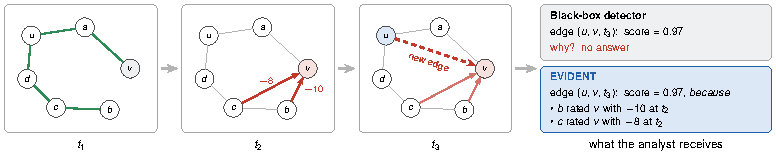
\includegraphics{Fig1.pdf}}
\caption{The problem, on a toy trust network. Green edges are positive ratings.
At $t_2$ two other traders rate trader $v$ negatively. At $t_3$ a new edge toward
$v$ appears, and it is anomalous because of what happened before, not because
$u$ and $v$ are strangers. Existing detectors return only a score for the new
edge. \evident{} returns the score together with the past interactions it was
computed from.}
\label{fig:motivation}
\end{figure*}

\textbf{Our answer.}
We present \evident{}, an intrinsically explainable detector built on a
sparse-evidence transformer. For each new edge, \evident{} gathers the recent
interactions of its two endpoints, selects a small subset of them as \emph{evidence}, and computes the anomaly score from
that subset and nothing else. The selected evidence is therefore the
explanation, and it is exact: no unselected token enters the computation. This is an architectural property, and it can be tested. If we
close every evidence gate, the score must become the same constant for every
edge. It does, in every real-label run we performed.

\evident{} is also the most accurate of the dynamic-graph detectors we
evaluate on real labels, the setting that decides whether a detector can be
used in practice. It reaches $0.8622$ AUC on Bitcoin-OTC and $0.7606$ on Bitcoin-Alpha, against
$0.6794$ and $0.5974$ for the best existing detector. This accuracy is not
bought at the expense of the standard benchmark. Under injection, \evident{}
stays within about $0.05$ AUC of the strongest detectors while reading only $20\%$
of its input, and with its full input the same architecture reaches $0.988$
on Bitcoin-OTC, above the injected AUC of every baseline on that graph.

Our contributions are:
\begin{itemize}
\item \textbf{A detector whose explanation is its input.} \evident{} scores an
edge from a selected set of about five evidence tokens. We prove, and check
in every real-label run, that the score depends on the selected tokens only.
\item \textbf{A training objective that makes the evidence matter.} A necessity
term penalizes the model whenever the evidence it \emph{rejected} is still
predictive. It more than doubles the advantage of selected over random
evidence on both datasets.
\item \textbf{Explainability that is measured, not illustrated.} We use three
quantitative tests of an explanation (empty-evidence AUC, rationale advantage
and evidence precision lift) and report them for every run. The existing
detectors do not produce explanations natively, so they offer nothing to test.
\item \textbf{A real-label evaluation of the state of the art.} We run StrGNN,
TADDY and SAD on real anomaly labels with identical splits, test edges and
metric code, and on injected anomalies as a control. All three fall far below
their injected-benchmark accuracy. We also document why, among the public
datasets we examined, only two dynamic graphs qualify for such an evaluation.
\item \textbf{Higher accuracy than the state of the art on real labels.}
\evident{} outperforms all three detectors on both datasets and all three
metrics, and it has by far the smallest gap between injected and real
anomalies. Against SAD, which receives the same labels and rating-derived
features, it leads by $0.16$--$0.18$ AUC.
\end{itemize}

Section~\ref{sec:related} reviews related work. Section~\ref{sec:prelim} gives
definitions and notation. Section~\ref{sec:method} describes \evident{}.
Section~\ref{sec:bench} defines the real-label benchmark and explains the
choice of datasets, and Section~\ref{sec:setup} gives the experimental
setup. Section~\ref{sec:results} reports the results and
Section~\ref{sec:conclusion} concludes.

% =============================================================================
\section{Related Work}
\label{sec:related}

\subsection{Anomaly Detection in Dynamic Graphs}
Early methods relied on hand-designed statistics of the graph
stream~\cite{akoglu2015,ranshous2015}. Deep methods learn the representation.
NetWalk~\cite{netwalk} learns node embeddings from random walks and clusters
them. AddGraph~\cite{addgraph} couples a graph convolutional
network~\cite{gcn} with a recurrent unit and attention. StrGNN~\cite{strgnn}
extracts the enclosing subgraph of each edge, labels its nodes by distance to
the two endpoints in the style of SEAL~\cite{seal}, and classifies the sequence
of subgraphs with a graph network~\cite{dgcnn} and a recurrent unit.
TADDY~\cite{taddy} encodes each node by diffusion-based and distance-based
positions and feeds a window of snapshots to a
transformer~\cite{vaswani2017}. SAD~\cite{sad} builds on temporal graph
attention~\cite{tgat} and adds a deviation loss~\cite{devnet} and a supervised
contrastive loss~\cite{supcon}, both of which consume anomaly labels.
SLADE~\cite{slade} learns from edge streams without labels through
self-supervision on a memory-based temporal model~\cite{tgn}, and
GeneralDyG~\cite{yang2025generaldyg} samples temporal ego-graphs so that one
detector generalizes across dynamic graphs. Our benchmark~\cite{nekka_survey} runs thirteen of these detectors under one
protocol.

Almost all of these papers evaluate on injected anomalies. The exceptions use
node-level state labels from interaction logs~\cite{jodie}, which mark a user's
state change rather than an anomalous edge. Our benchmark~\cite{nekka_survey}
first observed that a simple degree heuristic rivals deep detectors under
injection and collapses on real Bitcoin labels. The present paper turns that
observation into a controlled test: the three strongest detectors, real
edge-level labels, one shared split, and an injected control for each. The
recent BAG benchmark~\cite{hua2026bag}, which compares $25$ detectors on
injected and organic anomalies, likewise finds that most methods struggle on
organic anomalies.

Neighboring fields have reached the same suspicion. On static graphs,
BOND~\cite{bond} reports that many deep outlier detectors that do well on
injected outliers do poorly on organic ones, and GADBench~\cite{gadbench}
finds that tree ensembles with simple neighbor aggregation beat specialized
graph networks. In dynamic link prediction, a pure memorization baseline
rivals deep models once negative edges are sampled
realistically~\cite{poursafaei2022}. Our results extend this line to anomaly
detection in dynamic graphs, and add a detector built for the real task.

\subsection{Explaining Graph Models}
\emph{Post-hoc} explainers take a trained model and search for the part of the
input that best preserves its output. GNNExplainer~\cite{gnnexplainer} and
PGExplainer~\cite{pgexplainer} learn edge masks, SubgraphX~\cite{subgraphx}
searches over subgraphs, T-GNNExplainer~\cite{tgnnexplainer} does so for
temporal models, and Shapley-based methods~\cite{shap} attribute the score to
input parts. Recent explainers for temporal graph networks search for
counterfactual subgraphs~\cite{qu2025cody} or find the evolving subgraphs
behind a prediction without training~\cite{lu2026temgx}; like the earlier
ones, they explain a model after it has been trained, and they target
prediction tasks rather than anomaly detection. We have followed this route for dynamic-graph detectors, with
attribution methods for recurrent, transformer-based and other deep
detectors~\cite{nekka_dsta,nekka_xtaddy,nekka_amortised}. That work is what motivated the present design. A post-hoc
explanation can be tested and tuned for fidelity, but the detector underneath
still reads its entire input, so the explanation can never be more than an
approximation~\cite{rudin2019}. Attention weights have the same problem: a
token with low attention still influences the output~\cite{jain2019}.

\emph{Ante-hoc} (intrinsic) methods build the explanation into the model. In
text, rationale models select a subset of the input and predict from
it~\cite{lei2016}; ERASER~\cite{eraser} standardized their evaluation. On
static graphs, GSAT~\cite{gsat} injects stochasticity into attention to obtain
interpretable subgraphs, and SIGNET~\cite{signet} gives self-interpretable
graph-level anomaly detection. On temporal graphs, TGIB~\cite{seo2024tgib}
uses an information bottleneck to predict a link together with the past events
that justify it. \evident{} brings this idea to edge-level
anomaly detection on dynamic graphs, where the unit of explanation has to say
both \emph{who} and \emph{when}. It differs from these models in three ways:
its unit of evidence is a (node,\,event) pair rather than a word, an edge or a
subgraph; its selector is factorized into ``who'' and ``when'' marginals, so
the explanation has a readable temporal structure; and closed evidence is
removed from the computation rather than down-weighted, which makes the
empty-evidence test of Section~\ref{sec:scoring} exact.

\subsection{Sparse Selection}
Selecting a discrete subset is not differentiable. We use the hard-concrete
relaxation~\cite{l0}, built on the concrete
distribution~\cite{concrete,gumbel}, which produces exact zeros and ones while
keeping a gradient. Rationale models can fail in a specific way: the selector
and the predictor agree on an arbitrary code, and the selection stops being
informative~\cite{interlocking}. Our factorized selector and necessity
objective are designed against this failure.

% =============================================================================
\section{Preliminaries}
\label{sec:prelim}

\begin{definition}[Dynamic graph]
A dynamic graph is a stream of timestamped events
$\Ecal=\{e_j=(u_j,v_j,t_j,x_j)\}_{j=1}^{M}$ with $t_1\le t_2\le\dots\le t_M$,
where $u_j,v_j\in\Vcal$ are the source and destination nodes and $x_j$ is an
optional attribute of the event (here, a rating). We write $\Ecal_{<t}$ for
the events that occur strictly before time $t$, and $\Hcal_x(t)$ for the events
of $\Ecal_{<t}$ that involve node $x$.
\end{definition}

We work directly on the event stream. Unlike snapshot-based
detectors~\cite{strgnn,taddy}, we do not bin time, so the exact delay between
two events is available to the model.

\begin{definition}[Edge anomaly detection]
Given a new event $e^\ast=(u,v,t^\ast)$ and its history $\Ecal_{<t^\ast}$, an
anomaly detector outputs a score $s(e^\ast)\in\R$, where a larger score means
a more anomalous event. Each event has a binary label $y\in\{0,1\}$ used for
training and evaluation.
\end{definition}

\begin{definition}[Intrinsically explainable detection]
\label{def:exp}
A detector is intrinsically explainable if, for each event $e^\ast$, it outputs a
pair $(s,\Rcal)$ such that (i) $\Rcal$ is a subset of the candidate evidence
items available at $t^\ast$, each item being a past event seen from one of its
endpoints, together with the descriptors of that event and node, and (ii) the
score is a function of $\Rcal$ alone: changing or removing any candidate item
outside $\Rcal$ leaves $s$ unchanged. We call $\Rcal$ the \emph{evidence}.
\end{definition}

Condition~(ii) is what separates an explanation that \emph{is} the decision
from one that describes it. A post-hoc explainer returns a set $\Rcal$ but
cannot satisfy (ii), since the model it explains has already read everything.
Table~\ref{tab:notation} lists our notation.

\begin{table}[!t]
\caption{Notation.}
\label{tab:notation}
\centering
\footnotesize
\renewcommand{\arraystretch}{1.12}
\begin{tabular}{@{}ll@{}}
\toprule
Symbol & Meaning\\
\midrule
$\Ecal$, $\Vcal$ & event stream, node set\\
$e^\ast=(u,v,t^\ast)$ & event to be scored (target)\\
$\Ecal_{<t}$, $\Hcal_x(t)$ & events before $t$; those involving node $x$\\
$W$, $N$, $T$ & pool size: events, nodes, token slots\\
$\ell(x)\in\{0,1,2\}^2$ & role of pool node $x$ relative to $(u,v)$\\
$\mathbf{r}_x\in\R^4$ & reputation descriptor of node $x$ at $t^\ast$\\
$\mathbf{q}_k\in\R^3$, $\Delta_k$ & descriptor and age of pool event $k$\\
$z_{i,k}\in\R^d$ & token for node $i$ in event $k$\\
$\theta_{i,k}$ & gate logit of token $(i,k)$\\
$a_i$, $b_k$ & ``who'' and ``when'' logits\\
$m_{i,k}\in\{0,1\}$ & gate (1 = selected as evidence)\\
$\Rcal$ & evidence: tokens with $m_{i,k}=1$\\
$p$ & evidence budget (fraction of tokens kept)\\
$\alpha_i$, $\beta_k$ & ``who'' and ``when'' marginals\\
$s$, $s_c$ & score from evidence; from rejected tokens\\
$\pi$ & anomaly rate in the training set\\
$\sigma(\cdot)$ & logistic function\\
\bottomrule
\end{tabular}
\end{table}

% =============================================================================
\section{The EVIDENT Method}
\label{sec:method}

\subsection{Overview}
Fig.~\ref{fig:pipeline} shows the pipeline. For a target event \evident{}
(1)~collects a fixed-size \emph{evidence pool} from the recent history of the
two endpoints, (2)~turns the pool into \emph{tokens}, each of which names one
counterparty in one past event, (3)~\emph{selects} a small subset of tokens,
and (4)~computes the score with a transformer that reads only the selected
tokens. The output is the score together with the selected tokens. There is no
separate explanation module: the explanation is the set of inputs that the
scoring layers received.

\begin{figure*}[!t]
\centering
\adjustbox{max width=\textwidth}{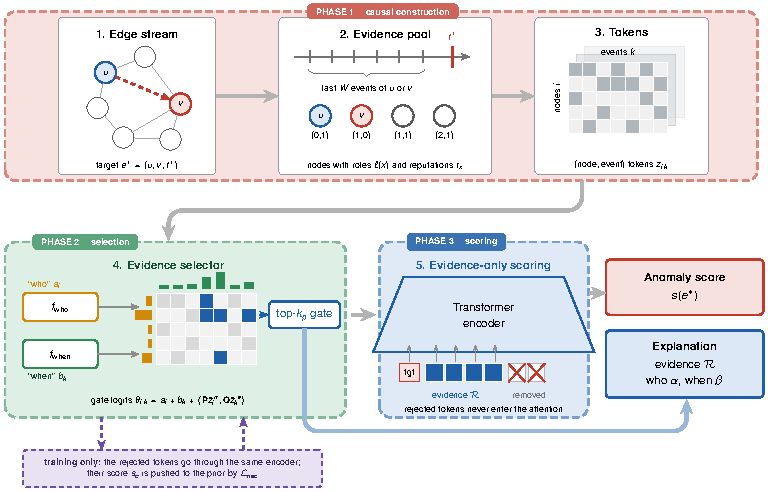
\includegraphics{Fig2.pdf}}
\caption{The \evident{} pipeline. \textbf{Top row, causal construction:} the
recent events of the two endpoints form a fixed-size evidence pool (1--2), and
every (node,\,event) pair in that pool becomes one token (3). \textbf{Bottom
row, selection and scoring:} a factorized selector scores each token from a
``who'' logit per node and a ``when'' logit per event, and opens a budget of
them (4, blue cells); a transformer then computes the anomaly score from the
open tokens and a constant target token, while rejected tokens are removed
from the computation rather than down-weighted (5). The open tokens, with the
two marginals, are returned as the explanation. During training only, the
rejected tokens are scored through the same encoder and penalized if they
remain predictive.}
\label{fig:pipeline}
\end{figure*}

\subsection{Evidence Pool}
For a target $e^\ast=(u,v,t^\ast)$, the pool holds the $W$ most recent events
of $\Hcal_u(t^\ast)\cup\Hcal_v(t^\ast)$ and their endpoints, capped at $N$
nodes with $u$ and $v$ always kept. Everything in the pool happened strictly
before $t^\ast$.

\emph{Roles.} Each pool node $x$ gets a double-radius label in the style of
enclosing-subgraph methods~\cite{seal,strgnn},
\begin{equation}
\ell(x)=\big(\min(\mathrm{dist}(x,u),2),\ \min(\mathrm{dist}(x,v),2)\big)\in\{0,1,2\}^2,
\label{eq:role}
\end{equation}
where $\mathrm{dist}$ is the hop distance in the graph of past events. The role says how
$x$ relates to the pair being scored, without using the identity of $x$.

\emph{Reputation.} Each pool node also carries a descriptor
$\mathbf{r}_x\in\R^4$ computed from $\Ecal_{<t^\ast}$: the log of its number
of past events, the mean rating it has received, the log of the number of
negative ratings it has received, and a flag for a node seen for the first
time. Each pool event $k$ carries a descriptor $\mathbf{q}_k\in\R^3$: its
rating, whether its source is one of the two target endpoints, and whether it
connects the same pair $\{u,v\}$. Its age is
$\Delta_k=\log(1+t^\ast-t_k)$, with $t_k$ its timestamp. All descriptors
are standardized with training-set statistics.

\emph{Nothing about the target itself is given to the model.} The rating of
$e^\ast$ defines its label, so it is never a feature. The model learns about
$e^\ast$ only through the history of its endpoints.

\emph{Fixed size.} Under injection, the size of the pool is itself a label
leak: two unrelated random nodes have little shared history, so their pool
looks different in size alone. We remove this shortcut from the input
representation by construction. Every
pool is resampled to exactly $N$ nodes, $W$ events and $T$ token slots, with
replacement when fewer are available~\cite{graphsage}, and duplicates are
masked so that they are never counted twice.

\subsection{Tokens}
A token is a valid (node, event) pair: token $(i,k)$ exists when node $i$ is
an endpoint of pool event $k$. This is the unit of explanation, and the choice
is deliberate. A node alone says who but not when. An event alone says when but
not who. A token says both: \emph{``counterparty $i$, in role $\ell_i$ and with
reputation $\mathbf{r}_i$, took part in an event of age $\Delta_k$ and rating
$x_k$''}. Its embedding is the sum of a node part and an event part,
\begin{equation}
z_{i,k}=\underbrace{E_{\text{role}}[\ell_i]+\mathbf{W}_n\mathbf{r}_i}_{\text{who}}
+\underbrace{\mathbf{w}_t\Delta_k+\mathbf{W}_e\mathbf{q}_k}_{\text{when and what}}
\ \in\R^{d},
\label{eq:token}
\end{equation}
where $E_{\text{role}}$ is an embedding table over the nine roles and
$\mathbf{W}_n,\mathbf{W}_e,\mathbf{w}_t$ are learned linear maps.

\subsection{Evidence Selector}
The selector decides which tokens become evidence. It uses its own, smaller
embeddings $\tilde{z}^{\,n}_i$ and $\tilde{z}^{\,e}_k$, built as
in~\eqref{eq:token} but with separate parameters, so that selecting and scoring
do not compete for the same representation. Two small networks give a ``who''
logit per node and a ``when'' logit per event,
\begin{equation}
a_i=f_{\text{who}}(\tilde{z}^{\,n}_i),\qquad
b_k=f_{\text{when}}(\tilde{z}^{\,e}_k),
\end{equation}
and the gate logit of a token is
\begin{equation}
\theta_{i,k}=a_i+b_k+\langle\mathbf{P}\tilde{z}^{\,n}_i,\ \mathbf{Q}\tilde{z}^{\,e}_k\rangle,
\label{eq:theta}
\end{equation}
with $\mathbf{P},\mathbf{Q}$ projecting to a small rank $r$.

This factorization does three jobs. First, it gives readable marginals,
$\alpha_i=\sigma(a_i)$ for \emph{which counterparty matters} and
$\beta_k=\sigma(b_k)$ for \emph{which moment matters}, as direct outputs of the
model. Second, it keeps the selector small. A free logit per token would give
the selector enough capacity to encode the label in the selection pattern,
which is the degenerate solution described in~\cite{interlocking}. Third, the
rank-$r$ term still lets a specific node matter at a specific time.

\emph{Gates.} During training, gates are sampled from the hard-concrete
distribution~\cite{l0}. With $\epsilon\sim\mathcal{U}(0,1)$, temperature $\tau$
and stretch limits $\gamma<0<1<\zeta$,
\begin{align}
\tilde{m}_{i,k}&=\sigma\!\Big(\tfrac{1}{\tau}\big(\log\epsilon-\log(1-\epsilon)
+\theta_{i,k}\big)\Big),\\
m_{i,k}&=\min\!\big(1,\max\!\big(0,\ \tilde{m}_{i,k}(\zeta-\gamma)+\gamma\big)\big).
\label{eq:gate}
\end{align}
At inference the gate is deterministic: the $k_p=\lceil p\,T'\rceil$ tokens
with the largest $\theta_{i,k}$ are opened, where $T'$ is the number of
distinct tokens in the pool and $p$ is the evidence budget.

\subsection{Evidence-Only Scoring}
\label{sec:scoring}
The scoring network is a transformer encoder~\cite{vaswani2017} that receives
a learned target token $z_\ast$ and the tokens of the pool. The score is read
from the target position,
\begin{equation}
s(e^\ast)=g\Big(\mathrm{Enc}\big(\{z_\ast\}\cup\{z_{i,k}:m_{i,k}=1\}\big)_{\ast}\Big),
\label{eq:score}
\end{equation}
with $g$ a two-layer perceptron. Two mechanisms together make a closed gate a
true removal:
\begin{itemize}
\item the token's vector is multiplied by its gate, so a closed token is the
zero vector;
\item its attention logit receives the bias $\log m_{i,k}$, which is $-\infty$
for a closed gate, so the token leaves every attention softmax.
\end{itemize}
The second mechanism is the one that is easy to get wrong. If a gate is floored
at a small value for numerical safety, a ``closed'' token still contributes a
tiny amount. AUC depends only on the ranking of scores, so a signal that is a
billion times smaller ranks the edges just as well. A model that attenuates
instead of removing behaves, under any ranking metric, as if no token had been
closed.

\begin{proposition}[Evidence-only scoring]
\label{prop:integrity}
At inference, the score~\eqref{eq:score} is a function of the selected tokens
$\Rcal=\{(i,k):m_{i,k}=1\}$ only. In particular, if $\Rcal=\emptyset$, then
$s(e^\ast)=c$ for a constant $c$ that is the same for all events, and the AUC
of the detector is exactly $0.5$.
\end{proposition}

\begin{proof}
A closed token has a zero value vector and an attention logit of $-\infty$, so
it contributes to no attention output at any layer, and the score is read at
the target position only. The target token $z_\ast$ is a learned constant that
receives no feature of $e^\ast$. With $\Rcal=\emptyset$, the encoder input is
the single constant token $z_\ast$, and so is its output. All events tie, and
the AUC of a constant score is $0.5$.
\end{proof}

Proposition~\ref{prop:integrity} is condition~(ii) of
Definition~\ref{def:exp}. It also gives a test that any implementation can
run: close every gate and measure AUC. We report this \emph{empty-evidence
check} for every run.

\subsection{Training Objective}
The loss has one detection term and five terms that shape the evidence,
\begin{equation}
\begin{split}
\Lcal={}&\Lcal_{\text{det}}+\lambda_{\text{nec}}\Lcal_{\text{nec}}
+\lambda_{\text{bud}}\Lcal_{\text{bud}}\\
&+\lambda_{\text{tv}}\Lcal_{\text{tv}}
+\lambda_{\text{stab}}\Lcal_{\text{stab}}+\lambda_{\text{ent}}\Lcal_{\text{ent}}.
\end{split}
\label{eq:loss}
\end{equation}

\emph{Detection.} $\Lcal_{\text{det}}$ is the binary cross-entropy between
$s$ and the label, with positives weighted by $(1-\pi)/\pi$. It is computed on
the gated pass only. At the operating budget the model is never trained with
all tokens open.

\emph{Necessity.} Let $s_c$ be the score obtained from the \emph{rejected}
tokens, i.e., with gate $1-m$. If the rejected tokens can still predict the
label, then the selected ones were not needed and the explanation is
arbitrary. We push the rejected-token score to the prior,
\begin{equation}
\Lcal_{\text{nec}}=\mathbb{E}\big[(s_c-\operatorname{logit}\pi)^2\big].
\label{eq:nec}
\end{equation}
A squared pull to a constant is used instead of a cross-entropy, because a
cross-entropy can be satisfied by an \emph{anti}-predictive score, which is
just as informative under a ranking metric.

\emph{Budget.} $\Lcal_{\text{bud}}=(\bar{m}-p)^2$, where $\bar{m}$ is the mean
probability that a gate is open, keeps the training density at the budget $p$
used at inference.

\emph{Temporal coherence.}
$\Lcal_{\text{tv}}=\frac{1}{W-1}\sum_k|\beta_{k+1}-\beta_k|$ discourages a
``when'' marginal that flickers between adjacent events.

\emph{Stability.} $\Lcal_{\text{stab}}=\mathbb{E}[(m-m')^2]$ for two
independent gate samples $m,m'$ penalizes a selector that returns a different
explanation each time it is asked.

\emph{Commitment.} $\Lcal_{\text{ent}}$ is the mean binary entropy of the
gate-open probabilities. Minimizing it pushes each gate toward a clear yes or
no, so that the top-$k_p$ selection at inference is not decided by noise.

\emph{Adaptive necessity weight.} A fixed $\lambda_{\text{nec}}$ is either too
weak to matter or strong enough to suppress detection. We adapt it once per
epoch. Let $\Lcal_{\text{triv}}=(1-\pi)\big(-\log\pi-\log(1-\pi)\big)$ be the
weighted detection loss of a model that outputs the prior $\pi$ for every
edge. If the detection loss is within $2\%$ of $\Lcal_{\text{triv}}$, detection
is being suppressed and $\lambda_{\text{nec}}$ is halved (not below $0.25$).
Otherwise, if the validation AUC of $s_c$ is more than $0.10$ away from $0.5$,
the rejected tokens are still informative and $\lambda_{\text{nec}}$ is
multiplied by $1.5$ (not above $8$).

\subsection{Algorithm and Cost}
Algorithm~\ref{alg:evident} summarizes scoring and training. One forward pass
returns the score, the evidence $\Rcal$, and the marginals $\alpha$ and
$\beta$. The explanation needs no second model and no extra pass.

The pool is built from per-node lists of recent events in $O(W)$ time. The
encoder attends over $T+1$ token slots, so scoring one edge costs
$O\big(L(T^2 d+T d^2)\big)$ for $L$ layers, which is a constant: it does not grow with the
size of the graph or with the length of the history. The total cost is linear
in the number of edges.

\begin{algorithm}[!t]
\caption{\evident{}: score and explain one event}
\label{alg:evident}
\begin{algorithmic}[1]
\Require target $e^\ast=(u,v,t^\ast)$; history $\Ecal_{<t^\ast}$; budget $p$;
flag \textsc{train}
\Ensure score $s$; evidence $\Rcal$; marginals $\alpha,\beta$
\Statex \rule{\linewidth}{0.4pt}
\Statex \textbf{Phase 1: causal, fixed-size evidence pool}
\State $\Pcal\gets$ last $W$ events of $\Hcal_u(t^\ast)\cup\Hcal_v(t^\ast)$
       \Comment{before $t^\ast$}
\State nodes $\gets$ endpoints of $\Pcal$, keeping $u$ and $v$, at most $N$
\State roles $\ell_i$; descriptors $\mathbf{r}_i,\mathbf{q}_k$; ages $\Delta_k$
       \Comment{from events before $t^\ast$ only}
\State $\Tcal\gets\{(i,k):\text{node } i \text{ is an endpoint of event } k\}$
\State resample to $(N,W,T)$; mask duplicates \Comment{no size leak}
\Statex \textbf{Phase 2: sparse evidence selection}
\State $z_{i,k}\gets$ token embeddings by~\eqref{eq:token}
\State $\theta_{i,k}\gets a_i+b_k+\langle\mathbf{P}\tilde{z}^{\,n}_i,
       \mathbf{Q}\tilde{z}^{\,e}_k\rangle$ \Comment{who $+$ when $+$ rank}
\If{\textsc{train}}
  \State $m,m'\gets$ two hard-concrete samples from $\theta$ by~\eqref{eq:gate}
\Else
  \State $m\gets$ open the $\lceil p\,T'\rceil$ tokens with largest $\theta$
\EndIf
\Statex \textbf{Phase 3: evidence-only scoring}
\State $s\gets g\big(\mathrm{Enc}(z_\ast,\{z_{i,k}:m_{i,k}=1\})_\ast\big)$
       \Comment{Proposition~\ref{prop:integrity}}
\Statex \textbf{Phase 4: training signal} \Comment{skipped at inference}
\If{\textsc{train}}
  \State $s_c\gets g\big(\mathrm{Enc}(z_\ast,\{z_{i,k}:m_{i,k}=0\})_\ast\big)$
  \State compute $\Lcal$ by~\eqref{eq:loss}; update parameters
  \State once per epoch: adapt $\lambda_{\text{nec}}$
\EndIf
\Statex \rule{\linewidth}{0.4pt}
\State $\Rcal\gets\{(i,k):m_{i,k}=1\}$;\ \ $\alpha\gets\sigma(a)$;\ \
       $\beta\gets\sigma(b)$
\State \Return $s,\ \Rcal,\ \alpha,\ \beta$ \Comment{one forward pass}
\end{algorithmic}
\end{algorithm}

% =============================================================================
\section{Real-Label Benchmark}
\label{sec:bench}

\subsection{Datasets With Real Labels}
We evaluate on Bitcoin-OTC and Bitcoin-Alpha~\cite{bitcoin1,bitcoin2}. Both
are who-trusts-whom networks of Bitcoin traders. Each event is a rating from
one trader to another on a scale from $-10$ (total distrust) to $+10$ (total
trust), written by a person who dealt with that trader. An event is
anomalous when its rating is at most $-5$, that is, in the strong-distrust
half of the negative scale. The threshold keeps the ratings that express
strong distrust and leaves out mildly negative ones, which can express a
minor complaint rather than an anomaly. Table~\ref{tab:data} gives
the statistics.

These labels are real in the sense that matters: nobody generated them for
the purpose of evaluation. A human being decided that the counterparty could
not be trusted and recorded it.

\begin{table}[!t]
\caption{Datasets. ``Usable'' events are those whose endpoints have at least
one earlier event. The split is chronological ($70/15/15$).}
\label{tab:data}
\centering
\footnotesize
\setlength{\tabcolsep}{4.5pt}
\begin{tabular}{@{}lrr@{}}
\toprule
 & Bitcoin-OTC & Bitcoin-Alpha\\
\midrule
Nodes & 5{,}881 & 3{,}783\\
Events & 35{,}592 & 24{,}186\\
Usable events & 35{,}511 & 23{,}692\\
Real anomalies (share of usable) & 2{,}660 (7.49\%) & 960 (4.05\%)\\
Train / val / test events & 24{,}857 / 5{,}327 / 5{,}327 & 16{,}584 / 3{,}554 / 3{,}554\\
Anomalies in train & 1{,}148 (4.62\%) & 544 (3.28\%)\\
Anomalies in test & 419 (7.87\%) & 227 (6.39\%)\\
\bottomrule
\end{tabular}
\end{table}

\subsection{Why Two Datasets: Real Edge-Level Labels Are Scarce}
\label{sec:whytwo}
Real-label evaluation is the core of this study, so we chose its data by rule
rather than by convenience. We fixed three requirements in advance and kept
every public dataset that meets all three.
\begin{enumerate}
\item \textbf{Real edge-level labels.} The label must mark an event, and it
must come from the real world rather than from an injection procedure.
\item \textbf{Recurring nodes.} A detector that reasons from history needs
nodes that appear more than once.
\item \textbf{Anomalies spread over time.} A chronological split must leave
anomalies in the training, validation and test periods.
\end{enumerate}
We examined six further public datasets that are widely used for dynamic
graphs or for anomaly detection. Each of them fails at least one requirement.
\begin{itemize}
\item \textbf{Wikipedia and MOOC}~\cite{jodie}: the label marks a change of
user state, not an anomalous event, and Wikipedia has only $217$ positives in
$157$k events.
\item \textbf{Elliptic}~\cite{elliptic}: each transaction appears in a single
time step, so no node has a history to reason from.
\item \textbf{CICIDS2017}~\cite{cicids}: the attacks arrive in scheduled
bursts, and a chronological split leaves no positive event in the test period.
\item \textbf{wiki-RfA}~\cite{wikirfa}: the closest structural match to the
Bitcoin networks, but $21.1\%$ of the votes are opposing ones, and an
opposing vote is an ordinary vote, not an anomaly.
\item \textbf{CTU-13}~\cite{ctu13}: in the capture we examined, a single
infected host emits every malicious flow, so counting the botnet flows a
source has already sent reaches $0.996$ AUC. The anomaly is a host, not an
event.
\end{itemize}
Among the public datasets we examined, Bitcoin-OTC and Bitcoin-Alpha are the
only dynamic graphs that satisfy all three requirements, which is why this study uses both
of them. This scarcity is itself a finding: the field has many dynamic graphs
but almost no real edge-level anomaly labels, and this is one reason why
evaluation has relied on injection. Our protocol, splits and code are public,
and we welcome any dynamic graph with real edge-level labels: it can be
evaluated under exactly the same protocol.

\subsection{Injected Anomalies as a Control}
To connect our results with the literature we also run the standard injected
protocol on the same two graphs. All real events are labeled normal. We then
add events between uniformly random node pairs, $5\%$ of the number of real
events, at timestamps drawn from the real ones, and label those anomalous. The
split and the evaluation code are the same as for real labels.

The control serves two purposes. It shows how each method behaves on the task
it was designed for, and it validates our implementation of each baseline: a
baseline that reaches its published level under injection but fails on real
labels has not been broken by our code.

\subsection{Split and Leakage Control}
Events are sorted by time and split $70/15/15$ into training, validation and
test. Every method is trained, selected and evaluated on the same three sets,
and all are scored on exactly the same test events. Every feature is computed
from events strictly earlier than the event being scored; counters are read
first and updated afterward.

% =============================================================================
\section{Experimental Setup}
\label{sec:setup}

\subsection{Baselines}
We compare with the three strongest detectors of our
benchmark~\cite{nekka_survey}, using the authors' code and published
hyperparameters. The other detectors of that benchmark, SLADE included, ranked
below these three.

\textbf{StrGNN}~\cite{strgnn} classifies the enclosing subgraph of an edge over
a window of five snapshots. Its original training draws negatives from
non-existent edges, which is only meaningful under injection. On real labels
we train it on the labeled training events; the architecture is unchanged.

\textbf{TADDY}~\cite{taddy} is trained as published, without labels, by
contrasting real edges with sampled negative edges.

\textbf{SAD}~\cite{sad} is semi-supervised: its deviation and contrastive
losses consume anomaly labels. We train it with all labels of the training
period. SAD expects edge features, and the Bitcoin graphs have none besides
the rating, so we give it four features computed from earlier events (the
prior degree of both endpoints, the mean rating the destination has received,
and its number of negative ratings). Without them SAD reaches only $0.5435$
AUC on Bitcoin-OTC, so the featured version is the one we report.

In short, \evident{}, StrGNN and SAD are trained on the anomaly labels of the
training period, and TADDY follows its label-free protocol. \evident{} and SAD
use information from past ratings; StrGNN and TADDY use topology and time only,
as designed. SAD is therefore the closest comparison: it receives the same labels as
\evident{} and rating-derived features of the same history. We also
report a parameter-free \textbf{degree} heuristic, which scores an edge by the
negated sum of its endpoints' degrees.

For every method the epoch is selected on validation AUC, and real-label
results are means over eight seeds (the seed counts under injection are given
with Table~\ref{tab:main}). StrGNN and TADDY use early stopping with a patience of
five evaluations.

\subsection{Implementation of EVIDENT}
One configuration is used for both datasets and both label regimes. The pool
holds $W=16$ events and $N=16$ nodes in $T=64$ token slots, and the evidence
budget is $p=0.20$. The encoder has $L=2$ layers, width $d=64$ and four
attention heads, and the selector has rank $r=4$; the model has $75{,}715$
parameters. The loss weights are $\lambda_{\text{bud}}=2$,
$\lambda_{\text{tv}}=0.05$, $\lambda_{\text{stab}}=0.10$ and
$\lambda_{\text{ent}}=0.01$, with $\lambda_{\text{nec}}$ starting at $1$ and
adapted within $[0.25,8]$. The gates use $(\tau,\gamma,\zeta)=(0.25,-0.1,1.1)$.
We train with AdamW~\cite{adamw} (learning rate $5\times10^{-4}$, weight decay
$10^{-5}$, batch size $64$) for $30$ epochs on a single NVIDIA T4 GPU; one run
takes about four minutes on Bitcoin-OTC.

\emph{Use of AI tools.} A large language model (Claude, Anthropic) was used to
assist with language editing, with the typesetting of figures, and with
writing code for parts of the experimental pipeline. The research idea, the
\evident{} method, the experimental design, the execution of all experiments,
and the analysis and interpretation of the results are the work of the
authors, who reviewed and verified all assisted material and take full
responsibility for the content of this article.

\subsection{Metrics}
\emph{Detection.} We report the area under the receiver operating characteristic curve (AUC), average
precision (AP), and precision among the $100$ highest-scored test events
(P@100). AP and P@100 matter because anomalies are rare: a detector can have
a decent AUC and still fill the top of its ranking with false
alarms~\cite{davis2006}.

\emph{Explanation.} We use three measurements.
\begin{itemize}
\item \textbf{Empty-evidence AUC.} The AUC with every gate closed. By
Proposition~\ref{prop:integrity} it must be $0.5$.
\item \textbf{Rationale advantage (RA).} The AUC obtained from the selected
evidence minus the AUC obtained from a \emph{random} set of tokens of the same
size. Comparing sets of equal size matters: the model is trained on small
inputs, so a comparison with a larger set would confound information with
input size.
\item \textbf{Evidence precision lift (EPL).} The share of selected tokens
whose past event carried a negative rating, divided by the same share for a
random set of the same size. A value above $1$ means the selector looks for
past distrust more often than chance.
\end{itemize}

% =============================================================================
\section{Results}
\label{sec:results}
We organize the results around six questions.
\begin{itemize}
\item \textbf{Q1.} How accurate are \evident{} and the existing detectors on
real labels?
\item \textbf{Q2.} What changes between injected and real anomalies?
\item \textbf{Q3.} Does \evident{} explain its decisions, and do the
explanations pass quantitative tests?
\item \textbf{Q4.} Which parts of \evident{} matter?
\item \textbf{Q5.} What does an explanation look like in practice?
\item \textbf{Q6.} How does \evident{} train, and what does it cost?
\end{itemize}

\subsection{Q1: Detection on Real Labels}
Table~\ref{tab:main} gives the main result. On real labels \evident{} is the
best method of the table on both datasets and on all three metrics.

\begin{table*}[!t]
\caption{Detection results on injected and on real labels (same graphs,
splits and metric code, and the same test events except where marked
$^{\ddagger}$). $\Delta$: AUC lost from injected to real, computed from
unrounded means; smaller is better. Real-label results are means $\pm$ one
standard deviation over eight seeds.
\textbf{Bold}: best real-label result and smallest $\Delta$. ``Labels'':
trained on the anomaly labels of the training period. ``Ratings'': reads the
ratings of past events.}
\label{tab:main}
\centering
\footnotesize
\setlength{\tabcolsep}{4.2pt}
\renewcommand{\arraystretch}{1.15}
\begin{adjustbox}{max width=\textwidth}
\begin{tabular}{@{}lcc ccccc ccccc@{}}
\toprule
 & & & \multicolumn{5}{c}{Bitcoin-OTC} & \multicolumn{5}{c}{Bitcoin-Alpha}\\
\cmidrule(lr){4-8}\cmidrule(l){9-13}
 & & & Injected & \multicolumn{4}{c}{Real labels}
     & Injected & \multicolumn{4}{c}{Real labels}\\
\cmidrule(lr){4-4}\cmidrule(lr){5-8}\cmidrule(lr){9-9}\cmidrule(l){10-13}
Method & Labels & Ratings & AUC & AUC & $\Delta$ & AP & P@100
       & AUC & AUC & $\Delta$ & AP & P@100\\
\midrule
Degree heuristic & -- & -- & 0.8841 & 0.4920 & 0.3921 & 0.0760 & 0.0100
                 & 0.8855 & 0.4269 & 0.4586 & 0.0580 & 0.0900\\
StrGNN~\cite{strgnn} & \checkmark & -- & 0.9819 & 0.5373\,$\pm$\,0.0190 & 0.4447 & 0.0874 & 0.0862
                 & 0.9775 & 0.5561\,$\pm$\,0.0154 & 0.4214 & 0.0751 & 0.0537\\
TADDY~\cite{taddy} & -- & -- & 0.9726 & 0.5390\,$\pm$\,0.0177 & 0.4336 & 0.0909 & 0.1175
                 & 0.9666 & 0.5570\,$\pm$\,0.0060 & 0.4097 & 0.0980 & 0.1837\\
SAD~\cite{sad} & \checkmark & \checkmark & 0.9779$^{\ddagger}$ & 0.6794\,$\pm$\,0.0070 & 0.2985 & 0.2183 & 0.3575
                 & 0.9443$^{\ddagger}$ & 0.5974\,$\pm$\,0.0140 & 0.3469 & 0.0997 & 0.1600\\
\midrule
\textbf{\evident{} (ours)} & \checkmark & \checkmark & 0.9614
                 & \textbf{0.8622}\,$\pm$\,0.0129 & \textbf{0.0991} & \textbf{0.5489} & \textbf{0.8650}
                 & 0.9271 & \textbf{0.7606}\,$\pm$\,0.0186 & \textbf{0.1665} & \textbf{0.2519} & \textbf{0.4163}\\
\bottomrule
\multicolumn{13}{@{}l}{\scriptsize Injected results: two seeds for StrGNN and
TADDY, four for SAD and \evident{}. $^{\ddagger}$Own draw of injected events,
same protocol.}
\end{tabular}
\end{adjustbox}
\end{table*}

On Bitcoin-OTC, \evident{} reaches $0.8622$ AUC. The best existing detector,
SAD, reaches $0.6794$, a gap of $0.18$. StrGNN and TADDY reach $0.5373$ and
$0.5390$, which is $0.32$ below \evident{} and only a few points above chance.
On Bitcoin-Alpha the picture is the same: $0.7606$ for \evident{} against
$0.5974$, $0.5570$ and $0.5561$.

The gap is even larger, in relative terms, on the metrics that describe the
top of the ranking. On Bitcoin-OTC, $86.5\%$ of the $100$ events that \evident{} ranks highest are
real anomalies; for SAD it is $35.8\%$, for TADDY $11.8\%$ and for StrGNN
$8.6\%$, close to the $7.9\%$ base rate. In average precision \evident{} is
$2.5\times$ above the best baseline on both datasets.

The differences are far outside seed noise: the worst \evident{} seed is above
the best seed of every baseline on both datasets. Welch's $t$-tests between \evident{} and each baseline give
$p<10^{-9}$ for AUC and $p<10^{-5}$ for AP in all six comparisons (three
baselines on two datasets), and every comparison remains significant after a
Bonferroni correction for the six tests.

\subsection{Q2: From Injected to Real Anomalies}
Fig.~\ref{fig:injreal} and the $\Delta$ columns of Table~\ref{tab:main} compare
the two label regimes. Under injection, every method looks excellent. StrGNN
and TADDY reach $0.97$--$0.98$, at or above their published level, and SAD
reaches $0.9779$ on Bitcoin-OTC (seed spread $0.0005$) and $0.9443$ on
Bitcoin-Alpha. This confirms that our implementations are sound: on injected
anomalies the three detectors reach the high accuracy reported for them on
injected benchmarks. Even the degree heuristic, which has no parameters,
reaches $0.88$: random node pairs can be recognized from graph structure
alone.

On real labels the same models, in the same code, lose $0.41$--$0.44$ AUC
for StrGNN and TADDY and $0.30$--$0.35$ for SAD. The degree heuristic drops below
chance. \evident{} loses $0.10$ on
Bitcoin-OTC and $0.17$ on Bitcoin-Alpha, by far the smallest loss, and keeps
$90\%$ and $82\%$ of its injected-benchmark AUC, against $55$--$58\%$ for
StrGNN and TADDY.

The consequence is that the two benchmarks tell different stories. Under
injection the four deep detectors lie within about $0.05$ AUC of one another, so the
injected benchmark cannot separate them. On real labels \evident{} leads StrGNN
and TADDY by $0.20$--$0.32$ and SAD by $0.16$--$0.18$. Injected accuracy alone
does not identify the detector that works on real anomalies.

\emph{Why the existing detectors fail on real labels.} They were designed
for, and tuned on, injected anomalies. An injected anomaly is a structural
event: two unrelated nodes connect. A real anomaly in a trust network is a
reputational event: the structure around it is ordinary, and the telling signs
are in the content of earlier interactions. StrGNN and TADDY read structure
and time only, so they see nothing unusual. \evident{} reads past interactions as
evidence tokens, ratings included, which is what a human analyst would do.

\emph{Competitive under injection by design.} \evident{} reads only $20\%$
of its pool, because a short explanation is the point of the model.
Section~\ref{sec:abl} shows that the same architecture reaches $0.988$ AUC
under injection once the budget is opened, above every baseline in
Table~\ref{tab:main}. This indicates that the small difference at $p=0.20$ is
mainly the price of an exact explanation rather than a limit of the
architecture, and we keep $p=0.20$ everywhere.

\begin{figure*}[!t]
\centering
\adjustbox{max width=\textwidth}{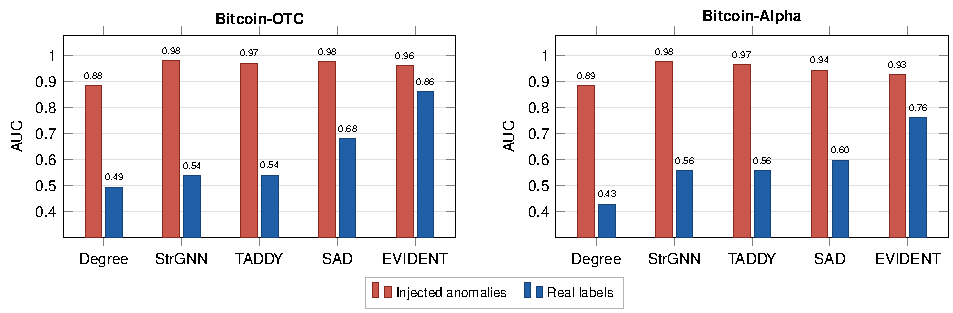
\includegraphics{Fig3.pdf}}
\caption{AUC on injected anomalies and on real labels, with the same graphs,
splits and code. Under injection all methods exceed $0.88$ and the four deep
detectors lie within about $0.05$ of one another. On real labels only \evident{}
stays far from chance.}
\label{fig:injreal}
\end{figure*}

\subsection{Q3: Measured Explainability}
\label{sec:explain}
Explainability is the second property that sets \evident{} apart, and we
measure it rather than illustrate it. Table~\ref{tab:explain} summarizes what
each method tells the analyst. StrGNN,
TADDY and SAD output a score only, so none of the explanation measurements
applies to them; the entries are not missing values but the absence of
anything to measure.

\begin{table}[!t]
\caption{Explainability. StrGNN, TADDY and SAD produce a score and no
explanation, so the measurements do not apply (\na). Values for \evident{} are
means over eight seeds, given as Bitcoin-OTC / Bitcoin-Alpha.}
\label{tab:explain}
\centering
\footnotesize
\setlength{\tabcolsep}{3.4pt}
\renewcommand{\arraystretch}{1.18}
\begin{tabular}{@{}lcccc@{}}
\toprule
 & StrGNN & TADDY & SAD & \textbf{\evident{}}\\
\midrule
Explains each score & no & no & no & \textbf{yes}\\
Says \emph{who} and \emph{when} & \na & \na & \na & \textbf{yes}\\
Score uses the evidence only & \na & \na & \na & \textbf{yes}\\
Empty-evidence AUC & \na & \na & \na & \textbf{0.5000 / 0.5000}\\
Evidence items per decision & \na & \na & \na & \textbf{4.7 / 4.6}\\
Rationale advantage & \na & \na & \na & \textbf{0.1336 / 0.0762}\\
Evidence precision lift & \na & \na & \na & \textbf{2.14$\times$ / 1.98$\times$}\\
Extra forward passes needed & \na & \na & \na & \textbf{none}\\
\bottomrule
\end{tabular}
\end{table}

\emph{The score depends on the evidence only.} With every gate closed, the AUC
of \evident{} is exactly $0.5000$ in all $32$ real-label runs behind
Tables~\ref{tab:main} and~\ref{tab:ablation}, in the $21$ runs of the
budget--width grid of Section~\ref{sec:abl}, and in $24$ further runs of a
sensitivity study that varied the budget, the width and the selection
criterion.
This is Proposition~\ref{prop:integrity} observed in practice.

\emph{The evidence is better than random evidence.} Scoring from the selected
tokens gives an AUC that is $0.1336$ (Bitcoin-OTC) and $0.0762$
(Bitcoin-Alpha) higher than scoring from the same number of random tokens.

\emph{The evidence is about distrust.} Selected tokens refer to a negatively
rated past event about twice as often as random tokens do ($2.14\times$ and
$1.98\times$), which is consistent with where an analyst would look.

\emph{The explanation is short.} A decision rests on $4.7$ distinct tokens on
average on Bitcoin-OTC and $4.6$ on Bitcoin-Alpha, out of about $20$ available
ones.

\emph{The evidence separates the two classes.} Fig.~\ref{fig:tsne} projects
the representation the score is read from, for the test events, to two
dimensions with t-SNE~\cite{tsne}. Real anomalies concentrate in part of the map instead of mixing
uniformly with the normal events, and by Proposition~\ref{prop:integrity} that
structure comes from the selected evidence alone. The separation is partial,
as AUC values of $0.86$ and $0.76$ imply, but it is produced by about five past
interactions per event.

\begin{figure}[!t]
\centering
\adjustbox{max width=\textwidth}{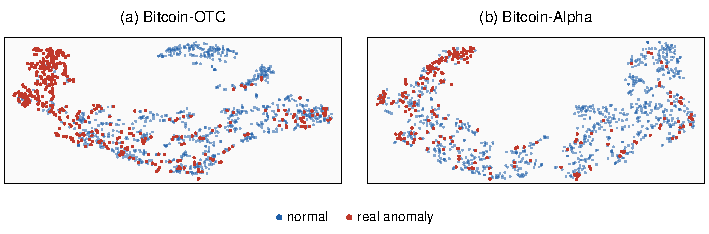
\includegraphics{Fig4.pdf}}
\caption{Two-dimensional t-SNE map of the vector the anomaly score is read
from, for the test events of one seed on (a) Bitcoin-OTC and (b)
Bitcoin-Alpha. By
Proposition~\ref{prop:integrity} that vector is a function of the selected
evidence alone, so the structure visible here is produced by about five past
interactions per event and nothing else. All test anomalies are shown; the
normal events are a random sample of $900$.}
\label{fig:tsne}
\end{figure}

\subsection{Q4: Ablation Study}
\label{sec:abl}
\emph{The necessity term.}
Table~\ref{tab:ablation} removes the necessity term
$\Lcal_{\text{nec}}$ and keeps everything else. Without it the selection still
happens and the score is still computed from the selected tokens, but the
selection carries little meaning: the rationale advantage more than halves on
Bitcoin-OTC ($0.1336\to0.0624$) and falls by about two thirds on Bitcoin-Alpha
($0.0762\to0.0269$), and the evidence precision lift falls to chance level or
below ($0.86$ and $1.02$). Both effects are significant on both datasets (paired $t$-test,
$p\le0.003$; Wilcoxon signed-rank, $p=0.008$).

This comes at a small cost in AUC ($0.014$ on Bitcoin-OTC and $0.034$ on
Bitcoin-Alpha), while AP and P@100 do not change significantly: a meaningful
explanation is cheap.

\emph{The evidence budget.} The budget $p$ sets how much of the pool the
scoring network may read, and it is the one knob that trades accuracy against
explanation. Fig.~\ref{fig:surface} maps that trade-off on real labels, over
seven budgets and three widths (one seed per cell). The rationale advantage
is highest for small budgets: at $d=64$ it stays between $0.20$ and $0.25$ up
to $p=0.20$, drops to $0.005$ at $p=0.75$, and is exactly zero at $p=1$, where
nothing is selected at all. Accuracy moves the other way at large budgets and
is highest at $p\ge0.75$ ($0.89$ at $d=64$). At $d=128$ accuracy is nearly
flat across budgets ($0.86$ to $0.89$), so at this width a small budget costs
little accuracy. Overall, opening the budget fully buys some
accuracy and costs the whole explanation. The same pattern holds under
injection, where AUC rises from $0.9730$ at $p=0.20$ to $0.9880$ at $p=1$ (one
seed each) as the rationale advantage falls from $0.1122$ to zero.
\evident{} runs at $p=0.20$ and $d=64$: budgets up to $0.20$ give the highest
rationale advantage, and $0.20$ leaves about five evidence items per decision
rather than one or two, which makes the explanation more informative for an
analyst. We use this setting unchanged in every other experiment and on both
datasets.

\begin{figure*}[!t]
\centering
\adjustbox{max width=\textwidth}{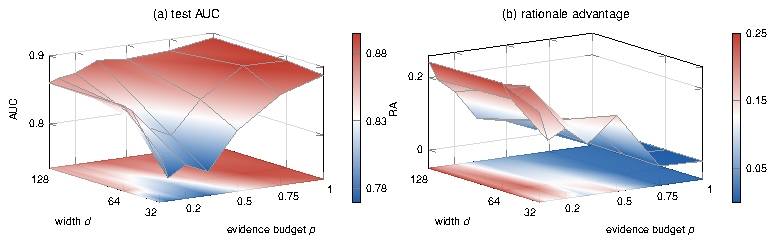
\includegraphics{Fig5.pdf}}
\caption{Sensitivity of \evident{} on Bitcoin-OTC over the evidence budget $p$
and the model width $d$ ($21$ trainings, one seed each, real labels; the
colored sheet on the floor repeats the surface). (a)~Accuracy is highest when
the budget is almost fully open. (b)~The rationale advantage falls to zero as
the budget opens: at $p=1$ nothing is selected and the model is a black box.
\evident{} operates at $p=0.20$, $d=64$, where the evidence is most
informative. With one seed per cell, single-cell differences are indicative
only; the eight-seed mean at the operating point is the $0.8622$ of
Table~\ref{tab:main}.}
\label{fig:surface}
\end{figure*}

\begin{table}[!t]
\caption{Effect of the necessity term (eight paired seeds). RA: rationale
advantage. EPL: evidence precision lift.}
\label{tab:ablation}
\centering
\footnotesize
\setlength{\tabcolsep}{3.6pt}
\begin{tabular}{@{}llccccc@{}}
\toprule
Dataset & Variant & AUC & AP & P@100 & RA & EPL\\
\midrule
\multirow{2}{*}{Bitcoin-OTC} & \evident{} & 0.8622 & 0.5489 & 0.8650 & \textbf{0.1336} & \textbf{2.14}\\
 & w/o necessity & 0.8766 & 0.5653 & 0.8738 & 0.0624 & 0.86\\
\midrule
\multirow{2}{*}{Bitcoin-Alpha} & \evident{} & 0.7606 & 0.2519 & 0.4163 & \textbf{0.0762} & \textbf{1.98}\\
 & w/o necessity & 0.7948 & 0.2652 & 0.4300 & 0.0269 & 1.02\\
\bottomrule
\end{tabular}
\end{table}

\subsection{Q5: A Case Study}
Fig.~\ref{fig:case} shows what \evident{} returns for one test event of
Bitcoin-OTC that it flags as anomalous: a rating of $-10$ from trader $4420$
to trader $5642$. The pool for this event holds thirteen distinct tokens.
\evident{} opens three. All three are ratings of $-10$ issued by the same
source to three other traders: one five minutes earlier and two within the
previous two seconds. The rejected tokens include the source's older positive
ratings, from $35$ to $155$ hours before.

The explanation is a burst of maximally negative ratings from one account
within minutes. That is a recognizable pattern, rating bombing, and an analyst
can check it directly against the rating history.

We inspected $50$ test events in this way, $25$ anomalous and $25$ normal.
For the anomalous ones, $38.0\%$ of the selected tokens refer to a negatively
rated past event, against $28.0\%$ of the rejected ones. For the normal ones
the relation reverses, $1.6\%$ against $4.4\%$: when there is nothing to find,
the selector does not go looking for distrust.

\begin{figure}[!t]
\centering
\adjustbox{max width=\textwidth}{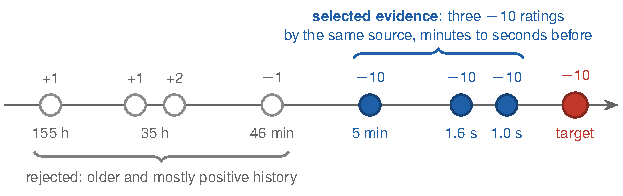
\includegraphics{Fig6.pdf}}
\caption{Explanation returned by \evident{} for a flagged event of
Bitcoin-OTC (a rating of $-10$ from trader $4420$ to trader $5642$). Circles
are past events in the evidence pool, placed in time order (not to scale),
with their rating above and their age below. Blue: selected as evidence.
White: rejected. Each past event contributes up to two (node,\,event) tokens,
one per endpoint.}
\label{fig:case}
\end{figure}

\subsection{Q6: Training and Cost}
\emph{Training and generalization over time.}
Fig.~\ref{fig:training}(a) shows validation AUC during training on
Bitcoin-OTC. \evident{} is above $0.93$ after the first epoch and stays there.
SAD climbs to about $0.85$. StrGNN rises to about $0.84$ and then declines as
it starts to overfit. TADDY never leaves the $0.55$--$0.60$ band.

Fig.~\ref{fig:training}(b) and (c) compare validation and test AUC. The test
period comes after the validation period, so the difference between the two
measures how well a detector carries over to the future. On Bitcoin-OTC,
StrGNN loses $0.29$ AUC between validation and test and SAD loses $0.17$,
against $0.09$ for \evident{}; on Bitcoin-Alpha the losses are $0.15$, $0.14$
and $0.10$. TADDY loses less, $0.06$ and $0.04$, but from a validation level
close to chance. Under injection this loss is zero or slightly negative for
StrGNN and TADDY, because a random pair looks the same in any period. The
larger loss on real labels suggests that real anomalies drift over time, which
is part of what makes the real task hard.

\begin{figure*}[!t]
\centering
\adjustbox{max width=\textwidth}{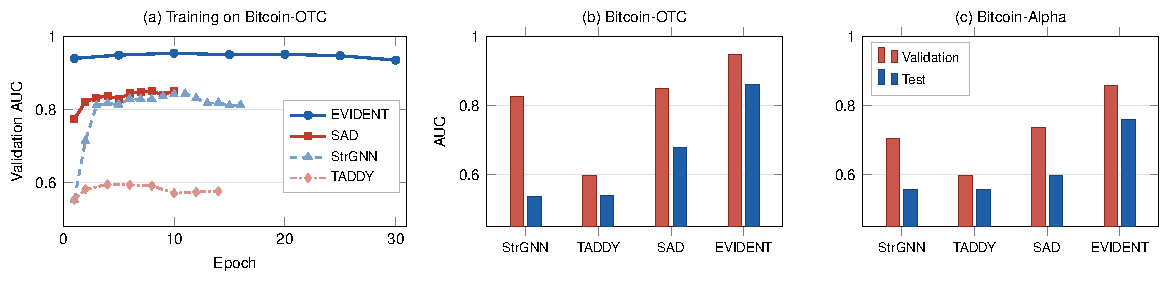
\includegraphics{Fig7.pdf}}
\caption{(a) Validation AUC during training on Bitcoin-OTC (seed~1 of each
method; \evident{} is logged every five epochs and TADDY about every two). (b,\,c) Mean validation and
test AUC on real labels over eight seeds. The test period follows the
validation period in time, so the drop from validation to test measures how
well each detector carries over to the future.}
\label{fig:training}
\end{figure*}

\emph{Cost.}
\evident{} has $75{,}715$ parameters. On a T4 GPU, scoring takes $0.026$~ms
per event in batches, and the time does not depend on the budget. Extracting
and returning the explanation adds $15.7\%$ to inference time on GPU and
$3.6\%$ on CPU; no extra forward pass is needed, because the explanation is a
by-product of the forward pass. Peak GPU memory
is $89$~MB. Training on Bitcoin-OTC takes about four minutes per run, against
$10$--$17$ minutes for StrGNN after a one-off subgraph extraction of about
$20$ minutes, about ten minutes for TADDY, and about six minutes for SAD.

% =============================================================================
\section{Conclusion}
\label{sec:conclusion}
Anomaly detectors for dynamic graphs are deployed on real anomalies, and their
alerts are acted on by people. We presented \evident{}, a sparse-evidence
transformer that scores each event from a small set of selected past
interactions and returns that set as the explanation. On real labels it
outperforms StrGNN, TADDY and SAD by $0.16$ to $0.32$ AUC and by at least
$2.5\times$ in average precision, on both datasets and all three metrics, and
it remains competitive on the injected benchmark. Its explanations are exact
by construction, short, better than random evidence and focused on past
distrust, and each of these properties is measured. We hope the
empty-evidence check and the real-label protocol used here become routine:
the first for any model that claims to be intrinsically explainable, the
second for any dynamic-graph detector that claims to be accurate.

Several directions follow from this work: a label-free variant of \evident{}
built on the same architecture, a study of its explanations with fraud
analysts, and new dynamic graphs with real edge-level labels, which would
benefit the whole field.

% =============================================================================
\backmatter

\section*{Declarations}

\begin{itemize}
\item \textbf{Funding.} The authors did not receive support from any
organization for the submitted work.
\item \textbf{Competing interests.} The authors have no competing interests
to declare that are relevant to the content of this article.
\item \textbf{Ethics approval and consent to participate.} Not applicable. The
study uses only publicly available, anonymized network data.
\item \textbf{Consent for publication.} Not applicable.
\item \textbf{Data availability.} Bitcoin-OTC and Bitcoin-Alpha are publicly
available from the Stanford Network Analysis Project at
\url{https://snap.stanford.edu/data/soc-sign-bitcoin-otc.html} and
\url{https://snap.stanford.edu/data/soc-sign-bitcoin-alpha.html}. The splits,
injected test sets and per-seed results are released with the code.
\item \textbf{Code availability.} Code, splits and per-seed results are
available at
\url{https://github.com/Iyad-Assaad-Nekka/EVIDENT-Explainable-Dynamic-Graph-anomaly-Detection}.
\item \textbf{Use of AI tools.} See the corresponding paragraph in
Section~\ref{sec:setup}.
\end{itemize}


% =============================================================================
\begin{thebibliography}{99}

\bibitem{akoglu2015}
Akoglu L, Tong H, Koutra D (2015) Graph based anomaly detection and description: a survey. Data Min Knowl Discov 29(3):626--688. \url{https://doi.org/10.1007/s10618-014-0365-y}

\bibitem{ranshous2015}
Ranshous S, Shen S, Koutra D, Harenberg S, Faloutsos C, Samatova NF (2015) Anomaly detection in dynamic networks: a survey. WIREs Comput Stat 7(3):223--247. \url{https://doi.org/10.1002/wics.1347}

\bibitem{ma2023}
Ma X, Wu J, Xue S, Yang J, Zhou C, Sheng QZ, Xiong H, Akoglu L (2023) A comprehensive survey on graph anomaly detection with deep learning. IEEE Trans Knowl Data Eng 35(12):12012--12038. \url{https://doi.org/10.1109/TKDE.2021.3118815}

\bibitem{ekle2024}
Ekle OA, Eberle W (2024) Anomaly detection in dynamic graphs: a comprehensive survey. ACM Trans Knowl Discov Data 18(8):192. \url{https://doi.org/10.1145/3669906}

\bibitem{bitcoin2}
Kumar S, Hooi B, Makhija D, Kumar M, Faloutsos C, Subrahmanian VS (2018) REV2: fraudulent user prediction in rating platforms. In: Proceedings of the 11th ACM International Conference on Web Search and Data Mining (WSDM). ACM, pp 333--341. \url{https://doi.org/10.1145/3159652.3159729}

\bibitem{netwalk}
Yu W, Cheng W, Aggarwal CC, Zhang K, Chen H, Wang W (2018) NetWalk: a flexible deep embedding approach for anomaly detection in dynamic networks. In: Proceedings of the 24th ACM SIGKDD International Conference on Knowledge Discovery \& Data Mining (KDD). ACM, pp 2672--2681. \url{https://doi.org/10.1145/3219819.3220024}

\bibitem{cicids}
Sharafaldin I, Lashkari AH, Ghorbani AA (2018) Toward generating a new intrusion detection dataset and intrusion traffic characterization. In: Proceedings of the 4th International Conference on Information Systems Security and Privacy (ICISSP). SciTePress, pp 108--116. \url{https://doi.org/10.5220/0006639801080116}

\bibitem{addgraph}
Zheng L, Li Z, Li J, Li Z, Gao J (2019) AddGraph: anomaly detection in dynamic graph using attention-based temporal GCN. In: Proceedings of the 28th International Joint Conference on Artificial Intelligence (IJCAI). IJCAI, pp 4419--4425. \url{https://doi.org/10.24963/ijcai.2019/614}

\bibitem{strgnn}
Cai L, Chen Z, Luo C, Gui J, Ni J, Li D, Chen H (2021) Structural temporal graph neural networks for anomaly detection in dynamic graphs. In: Proceedings of the 30th ACM International Conference on Information \& Knowledge Management (CIKM). ACM, pp 3747--3756. \url{https://doi.org/10.1145/3459637.3481955}

\bibitem{taddy}
Liu Y, Pan S, Wang YG, Xiong F, Wang L, Chen Q, Lee VCS (2023) Anomaly detection in dynamic graphs via transformer. IEEE Trans Knowl Data Eng 35(12):12081--12094. \url{https://doi.org/10.1109/TKDE.2021.3124061}

\bibitem{sad}
Tian S, Dong J, Li J, Zhao W, Xu X, Wang B, Song B, Meng C, Zhang T, Chen L (2023) SAD: semi-supervised anomaly detection on dynamic graphs. In: Proceedings of the 32nd International Joint Conference on Artificial Intelligence (IJCAI). IJCAI, pp 2306--2314. \url{https://doi.org/10.24963/ijcai.2023/256}

\bibitem{slade}
Lee J, Kim S, Shin K (2024) SLADE: detecting dynamic anomalies in edge streams without labels via self-supervised learning. In: Proceedings of the 30th ACM SIGKDD Conference on Knowledge Discovery and Data Mining (KDD). ACM, pp 1506--1517. \url{https://doi.org/10.1145/3637528.3671845}

\bibitem{nekka_survey}
Nekka IA, Seba H, Hidouci WK, Amrouche K (2026) Deep learning for anomaly detection in dynamic graphs: a verified taxonomy, survey, and unified benchmark. SSRN preprint. \url{https://papers.ssrn.com/sol3/papers.cfm?abstract_id=7339339}

\bibitem{gnnexplainer}
Ying R, Bourgeois D, You J, Zitnik M, Leskovec J (2019) GNNExplainer: generating explanations for graph neural networks. In: Advances in Neural Information Processing Systems 32 (NeurIPS). Curran Associates. \url{https://proceedings.neurips.cc/paper_files/paper/2019/file/d80b7040b773199015de6d3b4293c8ff-Paper.pdf}

\bibitem{pgexplainer}
Luo D, Cheng W, Xu D, Yu W, Zong B, Chen H, Zhang X (2020) Parameterized explainer for graph neural network. In: Advances in Neural Information Processing Systems 33 (NeurIPS). Curran Associates, pp 19620--19631. \url{https://proceedings.neurips.cc/paper/2020/hash/e37b08dd3015330dcbb5d6663667b8b8-Abstract.html}

\bibitem{tgnnexplainer}
Xia W, Lai M, Shan C, Zhang Y, Dai X, Li X, Li D (2023) Explaining temporal graph models through an explorer-navigator framework. In: Proceedings of the 11th International Conference on Learning Representations (ICLR). \url{https://openreview.net/forum?id=BR_ZhvcYbGJ}

\bibitem{nekka_dsta}
Nekka IA, Seba H, Hidouci WK, Amrouche K (2026) Dual spatial-temporal attribution: architecture-aligned post-hoc explainability for recurrent graph anomaly detection. arXiv preprint arXiv:2608.12441

\bibitem{nekka_amortised}
Nekka IA, Seba H, Hidouci WK, Amrouche K (2026) Amortised post-hoc explanation with exact preservation for dynamic graph anomaly detectors. arXiv preprint arXiv:2608.15559

\bibitem{nekka_xtaddy}
Nekka IA, Seba H, Hidouci WK, Amrouche K (2026) Dual spatial-temporal Shapley attribution for explainable anomaly detection in dynamic social networks. In: IEEE International Conference on Social Networks Analysis, Management and Security (SNAMS 2026). Accepted for publication

\bibitem{rudin2019}
Rudin C (2019) Stop explaining black box machine learning models for high stakes decisions and use interpretable models instead. Nat Mach Intell 1(5):206--215. \url{https://doi.org/10.1038/s42256-019-0048-x}

\bibitem{gcn}
Kipf TN, Welling M (2017) Semi-supervised classification with graph convolutional networks. In: International Conference on Learning Representations (ICLR)

\bibitem{seal}
Zhang M, Chen Y (2018) Link prediction based on graph neural networks. In: Advances in Neural Information Processing Systems 31 (NeurIPS), pp 5165--5175

\bibitem{dgcnn}
Zhang M, Cui Z, Neumann M, Chen Y (2018) An end-to-end deep learning architecture for graph classification. In: Proceedings of the 32nd AAAI Conference on Artificial Intelligence (AAAI). AAAI Press, pp 4438--4445. \url{https://doi.org/10.1609/aaai.v32i1.11782}

\bibitem{vaswani2017}
Vaswani A, Shazeer N, Parmar N, Uszkoreit J, Jones L, Gomez AN, Kaiser {\L}, Polosukhin I (2017) Attention is all you need. In: Advances in Neural Information Processing Systems 30 (NeurIPS), pp 5998--6008

\bibitem{tgat}
Xu D, Ruan C, Korpeoglu E, Kumar S, Achan K (2020) Inductive representation learning on temporal graphs. In: International Conference on Learning Representations (ICLR)

\bibitem{devnet}
Pang G, Shen C, van den Hengel A (2019) Deep anomaly detection with deviation networks. In: Proceedings of the 25th ACM SIGKDD International Conference on Knowledge Discovery \& Data Mining (KDD). ACM, pp 353--362. \url{https://doi.org/10.1145/3292500.3330871}

\bibitem{supcon}
Khosla P, Teterwak P, Wang C, Sarna A, Tian Y, Isola P, Maschinot A, Liu C, Krishnan D (2020) Supervised contrastive learning. In: Advances in Neural Information Processing Systems 33 (NeurIPS), pp 18661--18673

\bibitem{tgn}
Rossi E, Chamberlain B, Frasca F, Eynard D, Monti F, Bronstein M (2020) Temporal graph networks for deep learning on dynamic graphs. In: ICML 2020 Workshop on Graph Representation Learning and Beyond (GRL+). arXiv preprint arXiv:2006.10637

\bibitem{yang2025generaldyg}
Yang X, Zhao X, Shen Z (2025) A generalizable anomaly detection method in dynamic graphs. In: Proceedings of the AAAI Conference on Artificial Intelligence (AAAI), vol 39(20). AAAI Press, pp 22001--22009. \url{https://doi.org/10.1609/aaai.v39i20.35508}

\bibitem{jodie}
Kumar S, Zhang X, Leskovec J (2019) Predicting dynamic embedding trajectory in temporal interaction networks. In: Proceedings of the 25th ACM SIGKDD International Conference on Knowledge Discovery \& Data Mining (KDD). ACM, pp 1269--1278. \url{https://doi.org/10.1145/3292500.3330895}

\bibitem{hua2026bag}
Hua F, Qi Y, Wei Z, Tian Y, Xu C, Wu X, Li J, Guo J (2026) BAG: benchmarking anomaly detection on dynamic graphs. In: Proceedings of the AAAI Conference on Artificial Intelligence (AAAI), vol 40(17). AAAI Press, pp 14892--14900. \url{https://doi.org/10.1609/aaai.v40i17.38510}

\bibitem{bond}
Liu K, Dou Y, Zhao Y, et al (2022) BOND: benchmarking unsupervised outlier node detection on static attributed graphs. In: Advances in Neural Information Processing Systems 35 (NeurIPS), Datasets and Benchmarks Track, pp 27021--27035

\bibitem{gadbench}
Tang J, Hua F, Gao Z, Zhao P, Li J (2023) GADBench: revisiting and benchmarking supervised graph anomaly detection. In: Advances in Neural Information Processing Systems 36 (NeurIPS), Datasets and Benchmarks Track, pp 29628--29653

\bibitem{poursafaei2022}
Poursafaei F, Huang S, Pelrine K, Rabbany R (2022) Towards better evaluation for dynamic link prediction. In: Advances in Neural Information Processing Systems 35 (NeurIPS), Datasets and Benchmarks Track, pp 32928--32941

\bibitem{subgraphx}
Yuan H, Yu H, Wang J, Li K, Ji S (2021) On explainability of graph neural networks via subgraph explorations. In: Proceedings of the 38th International Conference on Machine Learning (ICML), PMLR 139, pp 12241--12252

\bibitem{shap}
Lundberg SM, Lee SI (2017) A unified approach to interpreting model predictions. In: Advances in Neural Information Processing Systems 30 (NeurIPS), pp 4765--4774

\bibitem{qu2025cody}
Qu Z, Gomm D, F\"arber M (2025) CoDy: counterfactual explainers for dynamic graphs. In: Proceedings of the 42nd International Conference on Machine Learning (ICML), PMLR, vol 267, pp 50762--50785. \url{https://proceedings.mlr.press/v267/qu25b.html}

\bibitem{lu2026temgx}
Lu M, Che H, Fan Y, Liu Q, Shao F, Ge T, Xiao X, Wu Y (2026) Training-free counterfactual explanation for temporal graph model inference. In: International Conference on Learning Representations (ICLR). \url{https://openreview.net/forum?id=NqtYz3A8tQ}

\bibitem{jain2019}
Jain S, Wallace BC (2019) Attention is not explanation. In: Proceedings of the 2019 Conference of the North American Chapter of the Association for Computational Linguistics: Human Language Technologies (NAACL-HLT), vol 1. Association for Computational Linguistics, pp 3543--3556. \url{https://doi.org/10.18653/v1/N19-1357}

\bibitem{lei2016}
Lei T, Barzilay R, Jaakkola T (2016) Rationalizing neural predictions. In: Proceedings of the 2016 Conference on Empirical Methods in Natural Language Processing (EMNLP). Association for Computational Linguistics, pp 107--117. \url{https://doi.org/10.18653/v1/D16-1011}

\bibitem{eraser}
DeYoung J, Jain S, Rajani NF, Lehman E, Xiong C, Socher R, Wallace BC (2020) ERASER: a benchmark to evaluate rationalized NLP models. In: Proceedings of the 58th Annual Meeting of the Association for Computational Linguistics (ACL). Association for Computational Linguistics, pp 4443--4458. \url{https://doi.org/10.18653/v1/2020.acl-main.408}

\bibitem{gsat}
Miao S, Liu M, Li P (2022) Interpretable and generalizable graph learning via stochastic attention mechanism. In: Proceedings of the 39th International Conference on Machine Learning (ICML), PMLR, vol 162, pp 15524--15543

\bibitem{signet}
Liu Y, Ding K, Lu Q, Li F, Zhang LY, Pan S (2023) Towards self-interpretable graph-level anomaly detection. In: Advances in Neural Information Processing Systems 36 (NeurIPS), pp 8975--8987. \url{https://doi.org/10.52202/075280-0394}

\bibitem{seo2024tgib}
Seo S, Kim S, Jung J, Lee Y, Park C (2024) Self-explainable temporal graph networks based on graph information bottleneck. In: Proceedings of the 30th ACM SIGKDD Conference on Knowledge Discovery and Data Mining (KDD). ACM. \url{https://doi.org/10.1145/3637528.3671962}

\bibitem{l0}
Louizos C, Welling M, Kingma DP (2018) Learning sparse neural networks through $L_0$ regularization. In: International Conference on Learning Representations (ICLR)

\bibitem{concrete}
Maddison CJ, Mnih A, Teh YW (2017) The concrete distribution: a continuous relaxation of discrete random variables. In: International Conference on Learning Representations (ICLR)

\bibitem{gumbel}
Jang E, Gu S, Poole B (2017) Categorical reparameterization with Gumbel-softmax. In: International Conference on Learning Representations (ICLR)

\bibitem{interlocking}
Yu M, Zhang Y, Chang S, Jaakkola T (2021) Understanding interlocking dynamics of cooperative rationalization. In: Advances in Neural Information Processing Systems 34 (NeurIPS)

\bibitem{graphsage}
Hamilton WL, Ying R, Leskovec J (2017) Inductive representation learning on large graphs. In: Advances in Neural Information Processing Systems 30 (NeurIPS), pp 1024--1034

\bibitem{bitcoin1}
Kumar S, Spezzano F, Subrahmanian VS, Faloutsos C (2016) Edge weight prediction in weighted signed networks. In: Proceedings of the IEEE 16th International Conference on Data Mining (ICDM). IEEE, pp 221--230. \url{https://doi.org/10.1109/ICDM.2016.0033}

\bibitem{elliptic}
Weber M, Domeniconi G, Chen J, Weidele DKI, Bellei C, Robinson T, Leiserson CE (2019) Anti-money laundering in Bitcoin: experimenting with graph convolutional networks for financial forensics. In: KDD '19 Workshop on Anomaly Detection in Finance. arXiv preprint arXiv:1908.02591

\bibitem{wikirfa}
West R, Paskov HS, Leskovec J, Potts C (2014) Exploiting social network structure for person-to-person sentiment analysis. Trans Assoc Comput Linguist 2:297--310. \url{https://doi.org/10.1162/tacl_a_00184}

\bibitem{ctu13}
Garc{\'\i}a S, Grill M, Stiborek J, Zunino A (2014) An empirical comparison of botnet detection methods. Comput Secur 45:100--123. \url{https://doi.org/10.1016/j.cose.2014.05.011}

\bibitem{adamw}
Loshchilov I, Hutter F (2019) Decoupled weight decay regularization. In: International Conference on Learning Representations (ICLR)

\bibitem{davis2006}
Davis J, Goadrich M (2006) The relationship between precision-recall and ROC curves. In: Proceedings of the 23rd International Conference on Machine Learning (ICML). ACM, pp 233--240. \url{https://doi.org/10.1145/1143844.1143874}

\bibitem{tsne}
van der Maaten L, Hinton G (2008) Visualizing data using t-SNE. J Mach Learn Res 9(86):2579--2605

\end{thebibliography}
\end{document}